\documentclass[11pt]{beamer}
\usetheme{Warsaw}
\usepackage[utf8]{inputenc}
\usepackage[english]{babel}
\usepackage{amsmath}
\usepackage{amsfonts}
\usepackage{amssymb}
\usepackage{color}
\usepackage{graphicx}
\definecolor{gray}{gray}{0.55}
\author{\textcolor{gray}{Adel Benamara} \and \textbf{Thomas Gougeon} \and \textbf{Ludovic
Robin} \\ \and Fred Raynal}

\AtBeginSection{\frame{\sectionpage}}
\title{Library version checking - QuarksLab \\ REDOCS'16}
%\setbeamercovered{transparent} 
%\setbeamertemplate{navigation symbols}{} 
%\logo{} 
%\institute{} 
%\date{} 
%\subject{} 
\begin{document}

\begin{frame}
\titlepage
\end{frame}

\begin{frame}
\tableofcontents
\end{frame}



%TODO : Detailler ce qu'on a fait
\section{Introduction}

\begin{frame}{Introduction}

    \begin{center}
    
\includegraphics[scale=0.38]{hacker.png}
    \end{center}

    \begin{block}{}
        \begin{itemize}
            \item \textbf{Hackers} look for vulnerabilities in programs ;
            \item Sometimes, finding one allow them to make an exploit ;
            \item \textbf{Developers} try to fix vulnerabilities, publishing a patch ;
            \item \textbf{Users} install the patch to hopefully fix the vulnerability on
                their version of the program.
        \end{itemize}
    \end{block}
\end{frame}

\begin{frame}
    \frametitle{What could go wrong ?}
    \begin{center}
    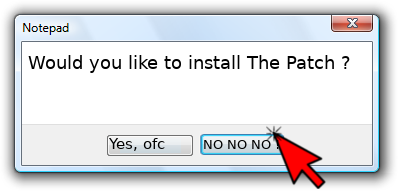
\includegraphics[scale=0.5]{box.png}
    \end{center}

    \begin{block}{}
    \begin{itemize}
        \item The vulnerability is not necessarily patched and the old version may remain ;
        \item \Huge Very \textcolor{red}{dangerous} !
    \end{itemize}
    \end{block}

    \end{frame}
    
    \begin{frame}{Which libraries are used by a program ?}
    
    	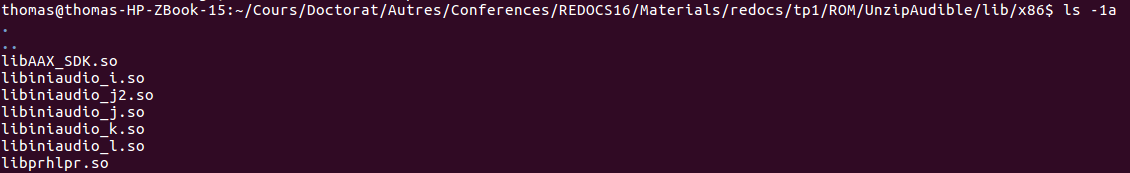
\includegraphics[scale=0.27]{s1.png}
    	~\\
    	~\\
    	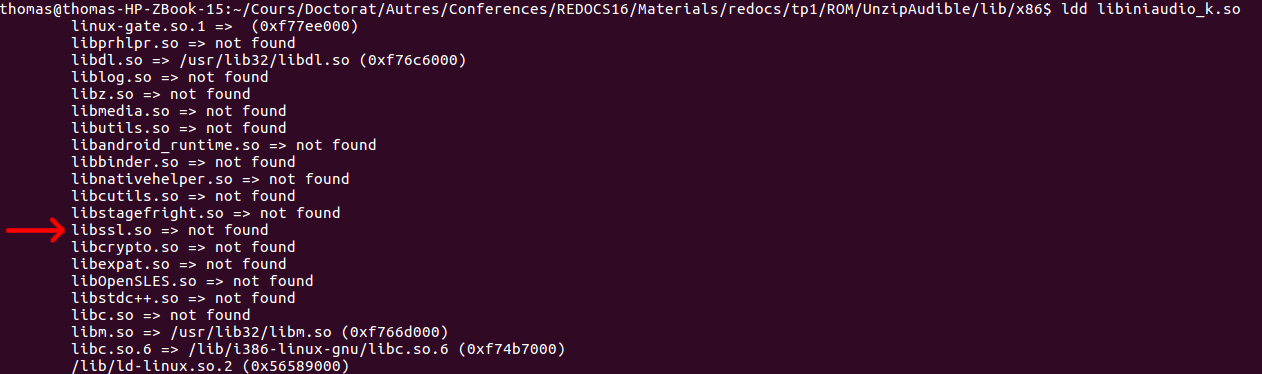
\includegraphics[scale=0.27]{s2.png}
    	
    	What is the version of OpenSSL ?
    \end{frame}
    
\begin{frame}
    \frametitle{Use your hands} 
    \begin{block}{Strings}
    	\begin{itemize}
    		\item Strings command gives binary infos.
    	\end{itemize}

    \end{block}
    \vspace{1em}
    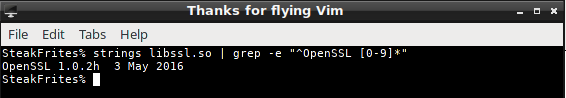
\includegraphics[scale=0.5]{strings.png}
    \vspace{1em}
    \begin{block}{It does not work for zlib}
    	\begin{itemize}
    		\item We do not know any other methods. But pros do.
    		\item Is there any pro here ?
    		
    	\end{itemize}

    \end{block}
     
\end{frame}

\section{Determine library version}

\begin{frame}
    \frametitle{Overview - How to check if we applied a patch ?}
   
    \begin{block}{What do we have ?}
        \begin{itemize}
            \item An unknown .so library, $L$ ;
            \item A set of known libraries sources, $S$.
        \end{itemize}
    \end{block}

    \begin{center}
        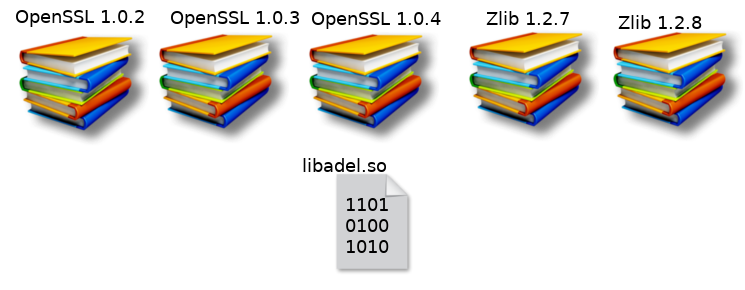
\includegraphics[scale=0.3]{bdd.png} 
    \end{center}

    \begin{block}{What are we doing ?}
        For all library $s$ in $S$, we check if $L$ is of the same version as $s$.
    \end{block}
\end{frame}





\begin{frame}
    \frametitle{Lazy start}

    
    \begin{block}{}
        \begin{itemize}
            \item Compile libraries in $S$, $c_1, \dots, c_n$ ; 
            \item Compare bit by bit $L$ and $c_1, \dots, c_n$.
        \end{itemize}
    \end{block}
    \begin{center}
    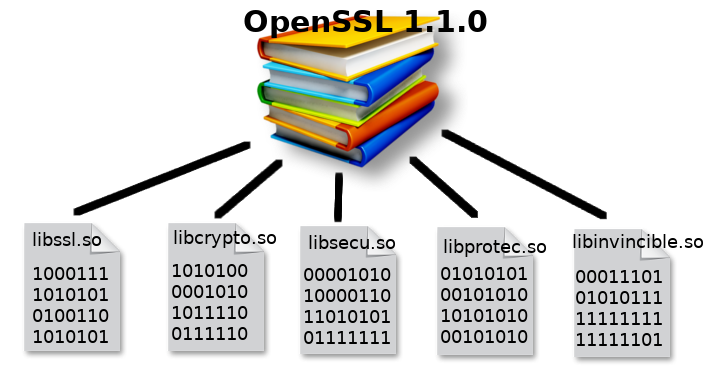
\includegraphics[scale=0.2]{compillib.png}
        \hspace{5em}
    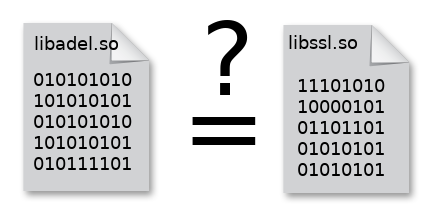
\includegraphics[scale=0.2]{compbin.png}
    \end{center}
    \begin{block}{Issues}
        $L$ is compiled with a different \textbf{compiler} and different \textbf{compiling options}.
    \end{block}

\end{frame}

\begin{frame}
    \frametitle{Be smarter}

    \begin{block}{Ideas}
    \begin{itemize}
        \item Link compatibility ;
        \item Malware signature ;
        \item Traces.
    \end{itemize}
    \end{block}
    \vspace{-0.8em}
    \begin{center}
        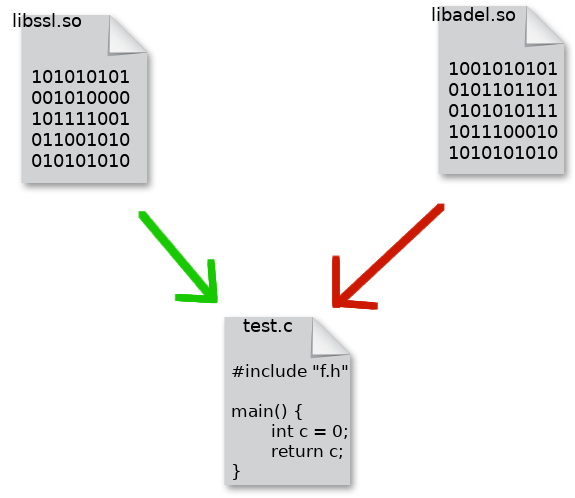
\includegraphics[scale=0.2]{link.png}
    
\includegraphics[scale=0.4]{malware.jpeg}
    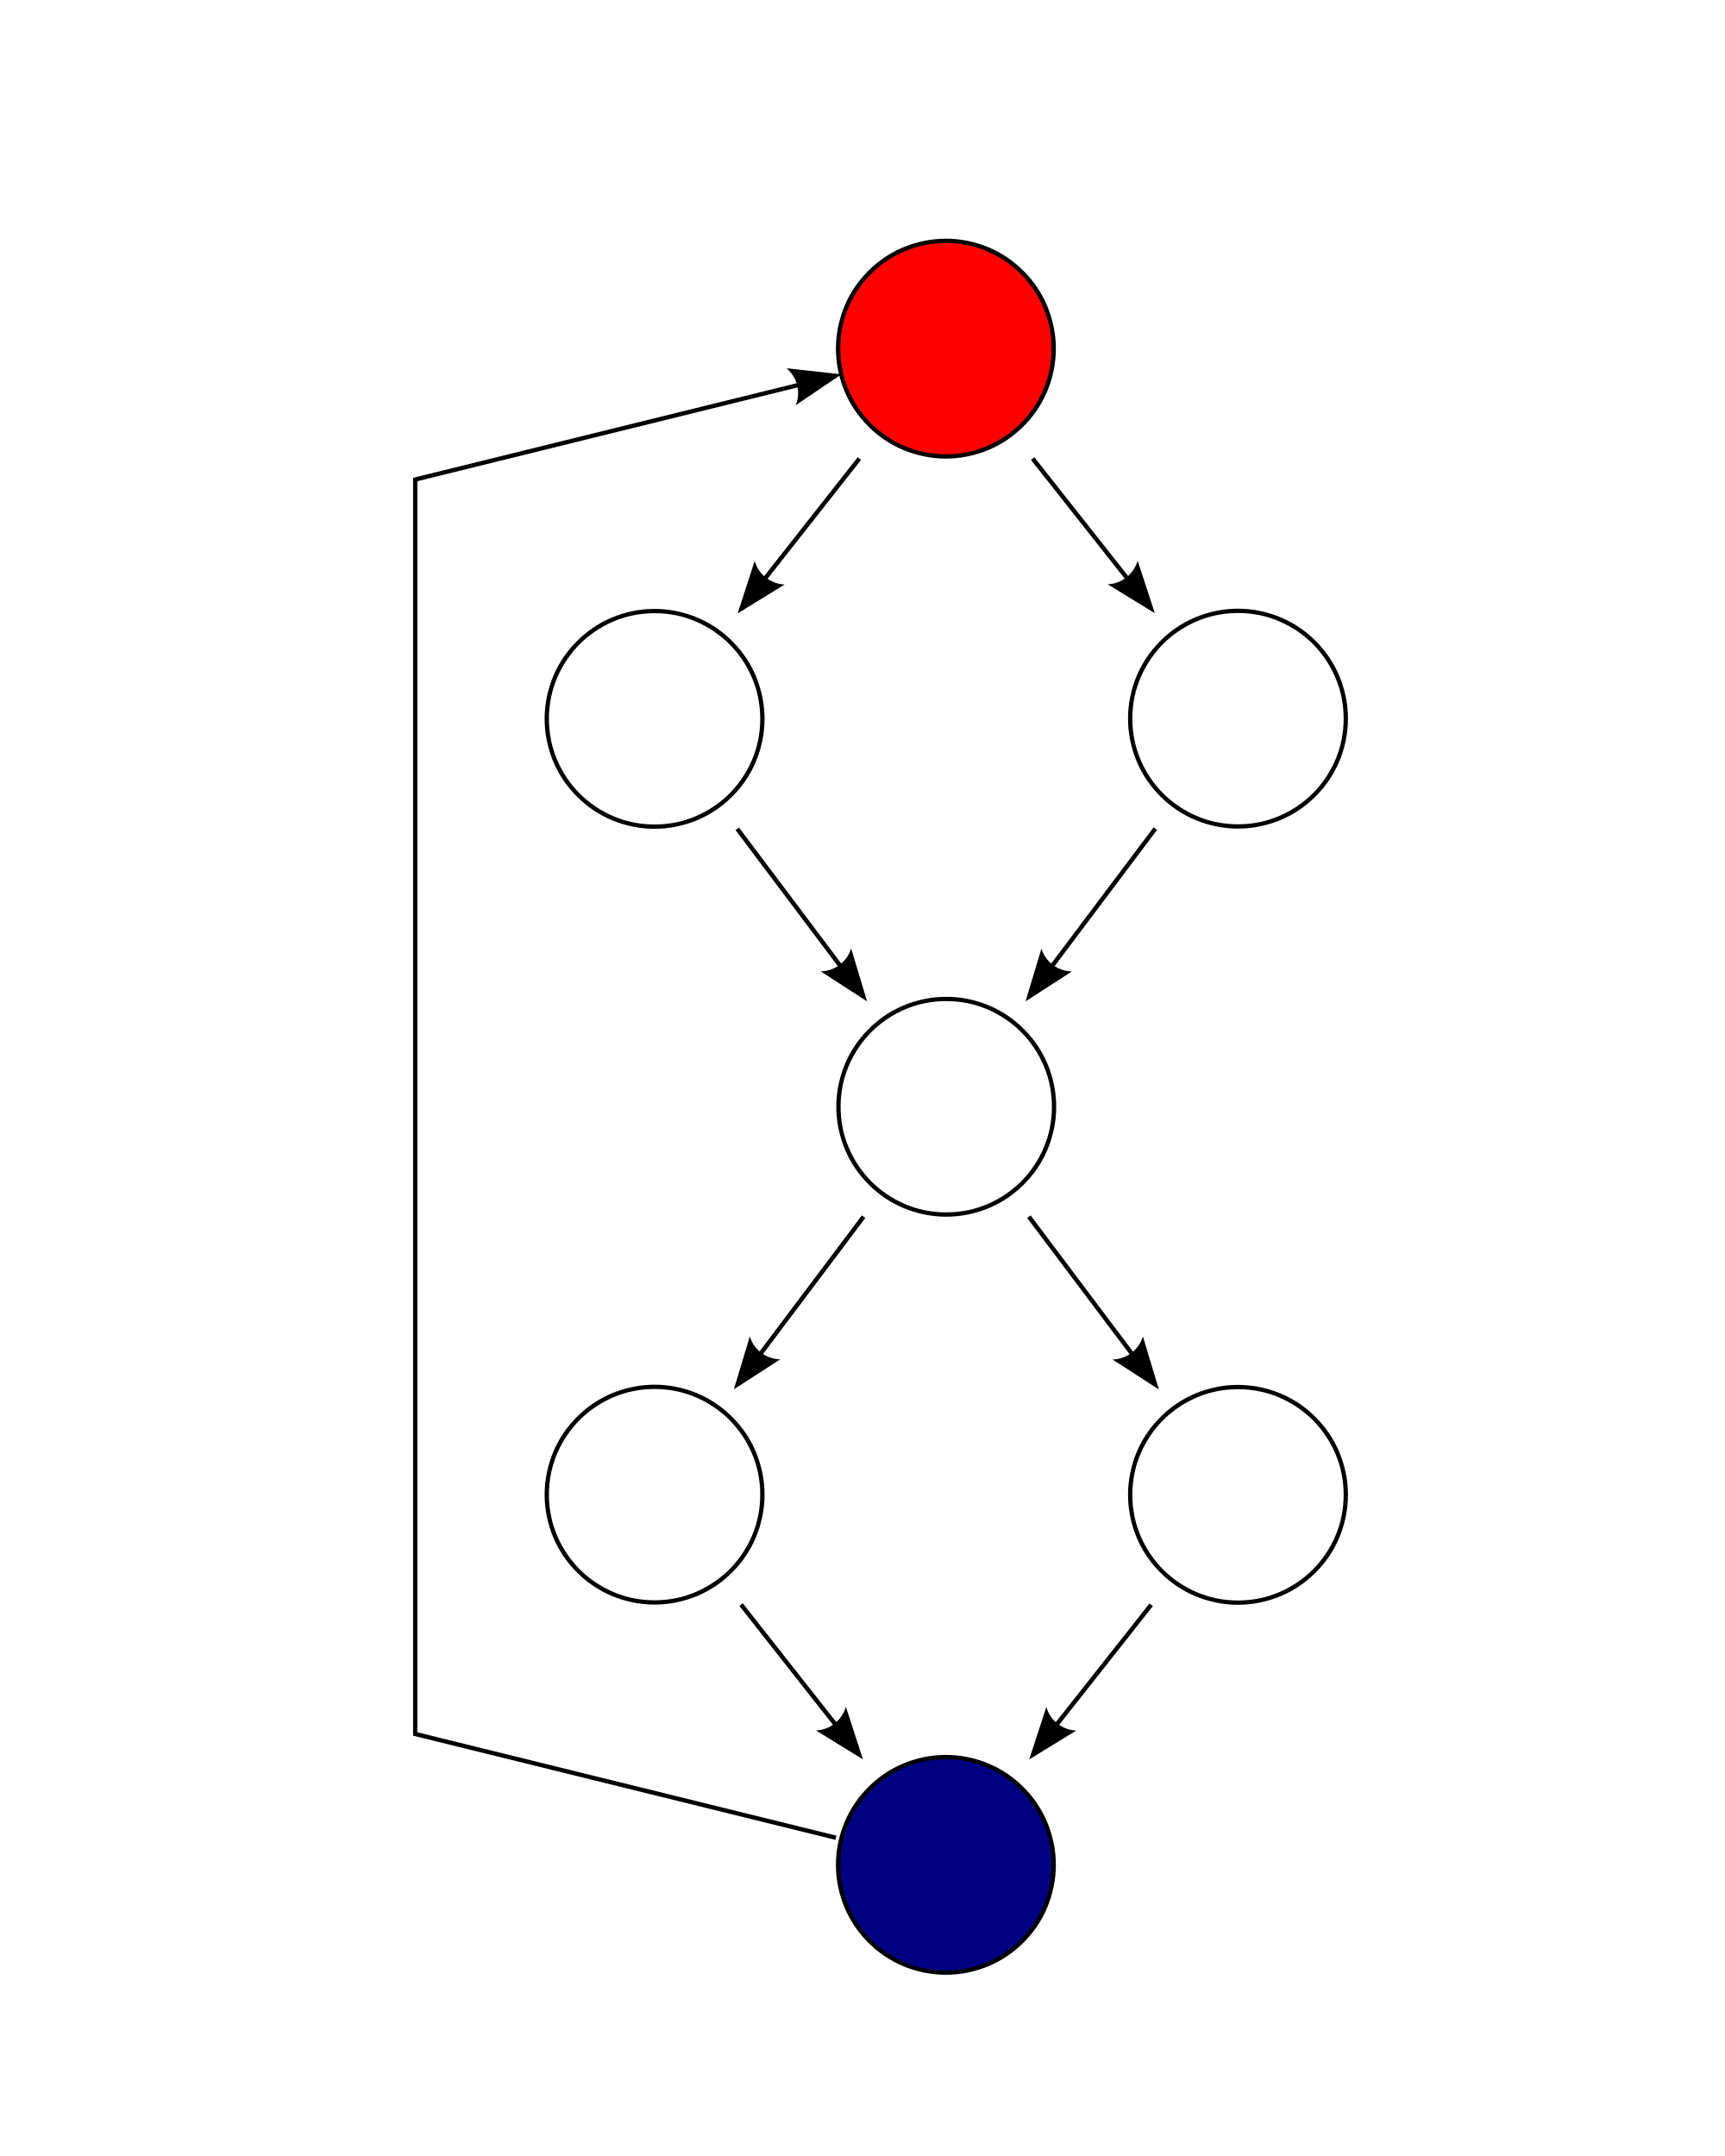
\includegraphics[scale=0.05]{cfg.png}
    \end{center}

\end{frame}

\begin{frame}
    \frametitle{Link dynamically the library}
    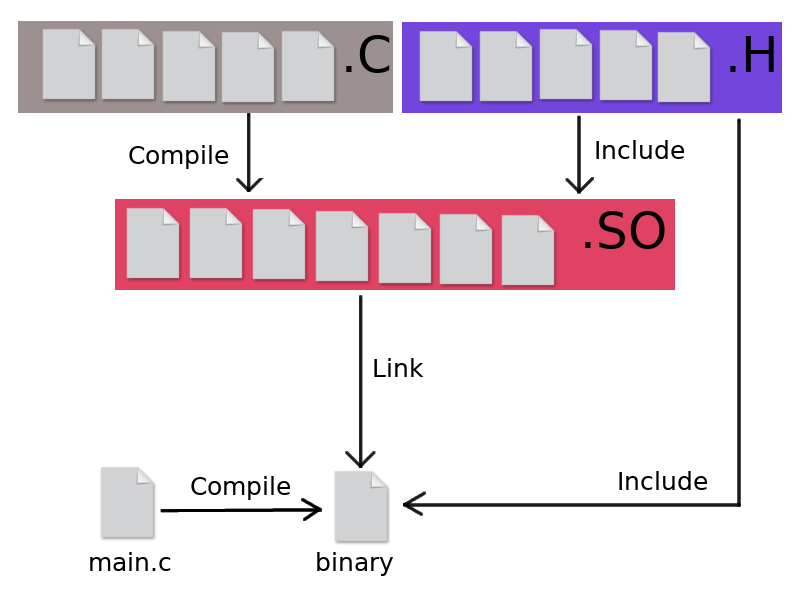
\includegraphics[scale=0.36]{compil1.png}
\end{frame}

\begin{frame}
    \frametitle{Link dynamically the library}
    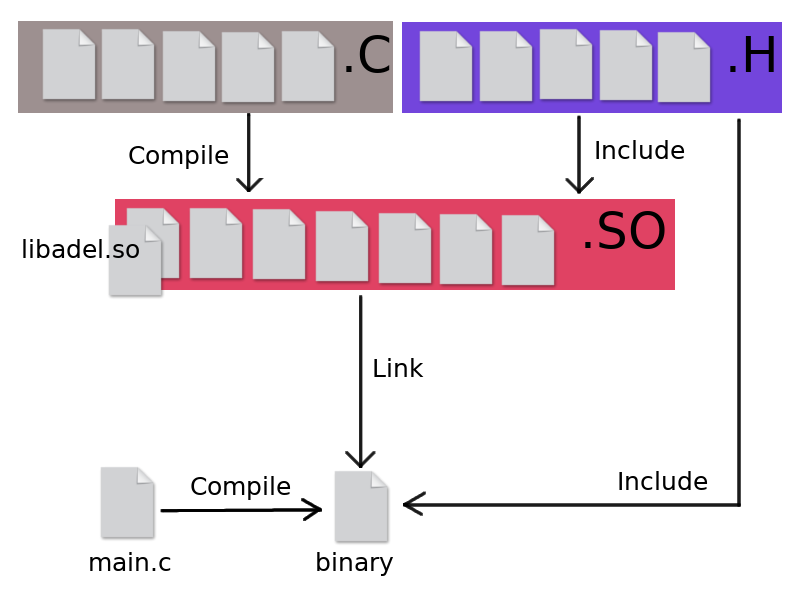
\includegraphics[scale=0.36]{compil2.png}
\end{frame}

\begin{frame}{What do we need ?}

	\begin{block}{Scripts}
		\begin{itemize}
			\item Generate .so from libraries: OpenSSL, Zlib, libXml, \dots
			\item Generate different versions for each library;
			\item Generate test program calling library functions;
			\item Link program with unknown library.
		\end{itemize}
	\end{block}
	

\end{frame}

\begin{frame}
    \frametitle{Turnkey programs} 
    \begin{block}{Build the program}
        \begin{itemize}
        	\item Checking major version of a library with link-testing;
        	\begin{itemize}
	            \item Semi-auto-compiling libraries ;
	            \item Semi-auto-extracting headers ;
    	        \item Auto-generation of a c program to link-test libraries.
        	
        	\end{itemize}
        \end{itemize}
    \end{block}

    \begin{block}{Tested with OpenSSL 1.0.2h}
        \begin{itemize}
            \item OpenSSL 1.0.2j - cannot distinguish; 
            \item OpenSSL 1.0.1e - can distinguish.
        \end{itemize}
    \end{block}

    \begin{block}{Tested with Zlib 1.2.8}
        \begin{itemize}
            \item Zlib 1.2.7 - cannot distinguish; 
            \item Zlib 1.1.3- can distinguish.
        \end{itemize}
    \end{block}

\end{frame}

\begin{frame}
    \frametitle{Malware signature}
    
    \begin{block}{Control flow graph}
    	\begin{itemize}
    		\item Representing binary with a CFG;
    		\item Using reduced CFG (Gorille);
    		\item Should work for major versions;  	
    		\item Not adapted to distinguish minor versions.
    	\end{itemize}
    \end{block}
    
    \begin{block}{Open questions}
    	\begin{itemize}
    		\item Distinguish minor patch from optimisation ?
    		\item How security patch more impacts binaries ?
    	\end{itemize}
    \end{block}
    
\end{frame}

\begin{frame}
    \frametitle{Analyse traces}
    \begin{block}{}
    	\begin{itemize}
    		\item Analyse program behaviour;
    		\item Analyse functions.

    	\end{itemize}
    \end{block}
    
    \begin{block}{Fuzzing}
    	\begin{itemize}
    		\item Does not work with references;
    		\item Smart fuzzing would be to use library tests.
    	\end{itemize}
    \end{block}
    
    \begin{block}{DSE}
    		Should work to distinguish functions

    \end{block}
    
\end{frame}







\section{Conclusion}

\iffalse
\begin{frame}{Find other execution paths}

\begin{block}{Coccinelle}
	\begin{itemize}
		\item Find known bugs in source code;
		\item Analyse patterns in source;
		\item Issue: We deal with binaries;
		\item Useful to find other execution paths for root cause.
	\end{itemize}
\end{block}

\end{frame}
\fi

\begin{frame}{Conclusion}

	\begin{block}{Issues}
		\begin{itemize}
			\item Tools are too specific to some cases, not our cases.
		\end{itemize}
	\end{block}

	\begin{block}{Results}
		\begin{itemize}
			\item Distinguish major versions ;
            \item Some ideas to improve results.
		\end{itemize}
	\end{block}
\end{frame}


\begin{frame}{It brought us..}


\begin{block}{Feelings}
	\begin{itemize}
		\item Inner peace;
        \item Intimacy;
        \item We lost faith in formal methods, for binary analysis at least.
	\end{itemize}
\end{block}

\begin{block}{Technical}
	\begin{itemize}
        \item We got back our Perl, that is priceless;
		\item Binaries are complex but fun.
	\end{itemize}
	
\end{block}

\end{frame}
\end{document}
